\documentclass{article}

% these packages let you do math
\usepackage{amsmath}
\usepackage{amssymb}

% we need these packages for fancy R tables
\usepackage{booktabs}
\usepackage{float}
\usepackage{colortbl}
\usepackage{xcolor}

% these packages play with the spacing/margins of the document. Uncomment the commands on lines 16 and 17 to see what they do.
\usepackage{a4wide}
\usepackage{setspace}
\usepackage{geometry}
\usepackage{parskip}
%\doublespacing
%\geometry{margin=1.5in}

% this package helps us with including images. Setting the graphics path makes it easier to refer to things in the \includegraphics command.
\usepackage{graphicx}
\graphicspath{ {../figures/} }

% make some hyperlinks using the \href command
\usepackage{hyperref}
\hypersetup{
    colorlinks=true,
    linkcolor=black,
    urlcolor=blue
}

% set the author, title, and date of the document. \maketitle adds it to the document.
\author{Sonali Mishra}
\title{Preliminary Analysis of Incarceration by Race and Gender}
\date{Spring 2022}

\begin{document}
\maketitle

\section{Overview}

This paper does a prima facie analysis of incarceration duration in United States in the year 2002 faceted at race and gender level. The way we calculate duration is by looking at \href{https://www.nlsinfo.org/investigator/pages/search}{NLS investigator}. We look at NLSY97 from 1997 to 2019 and download the incareration history captured for the year 2002. This dataset contains month-wise data and observations are recorded at individual level. Upon some data manipulation, we only consider the months when the individual was incarcerated in that month partially of entirely. We also have indicators on race (black, hispanic, mixed race and non-black. 

\section{Graphical representation}

The belore graph compares the length of incarceration between male and female across thnic groups. Black men spend roughly 8 times more time incarcerated than black women. The other two groups have similar trend except for mixed race (which is a data glitch perhaps). The way we look at the incarceration rate is number of individuals incarcerated as a proportion of 100,000 individuals. We look at this definition is because it is the most frequently used metric in discussions pertaining to this forum.

\begin{figure}[H]
    \begin{center}
        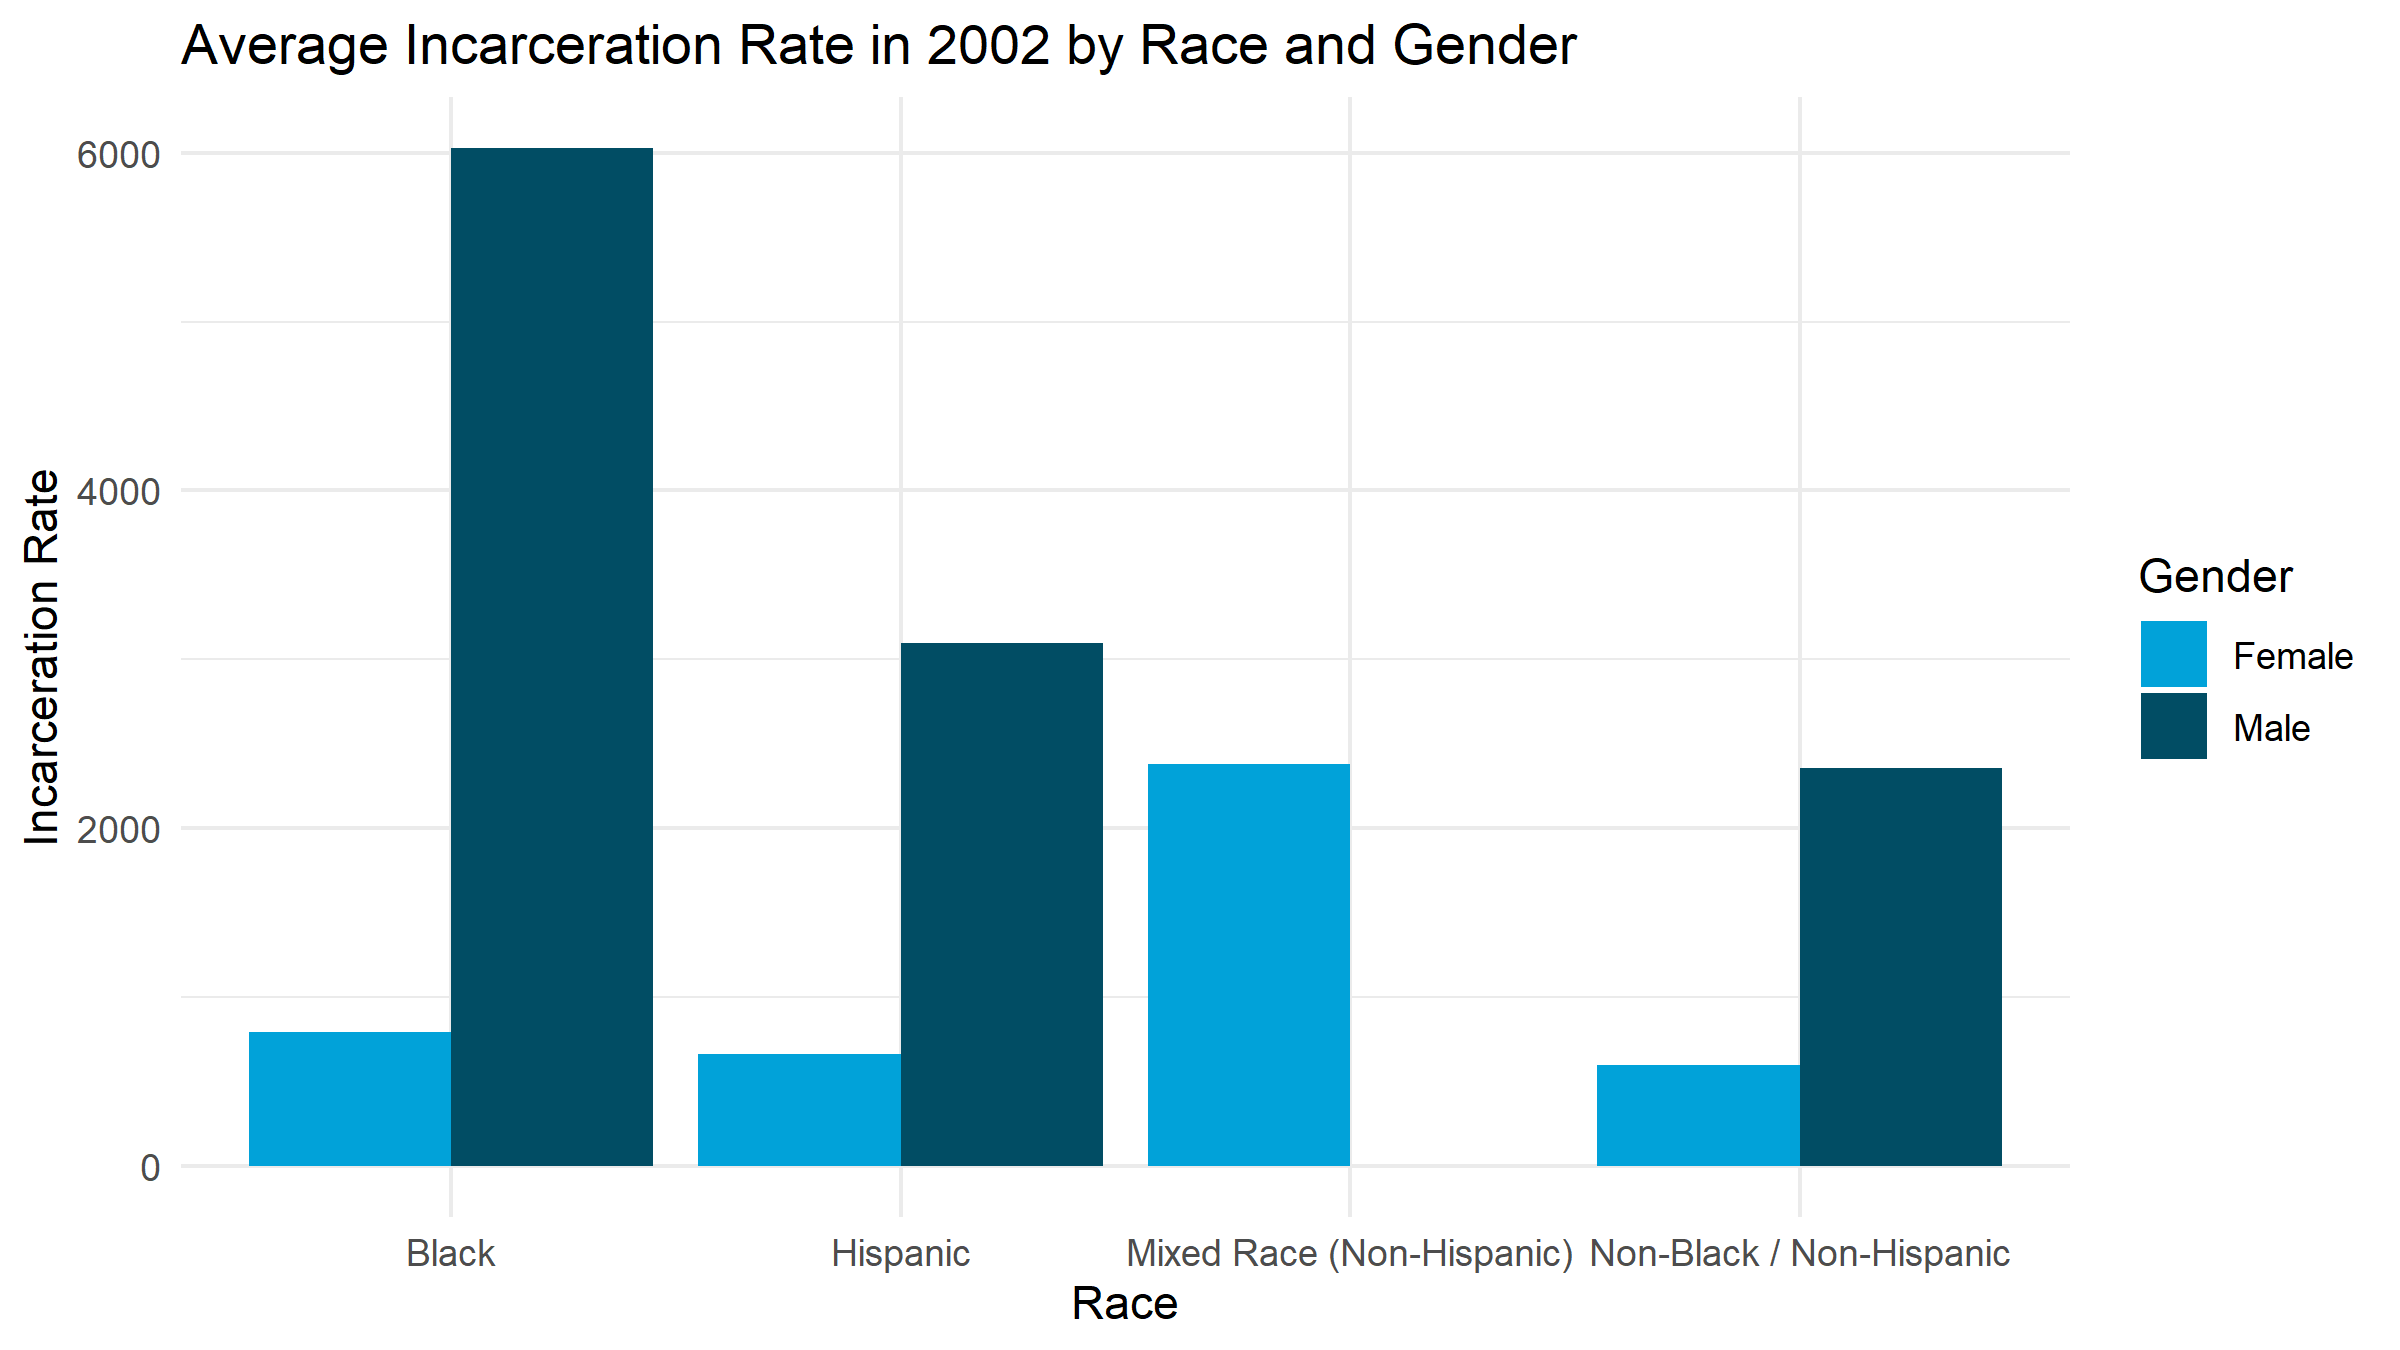
\includegraphics[width=.85\textwidth]{incar_rate_by_racegender}
    \end{center}
    \caption{Incarceration Rate on an average (for a given 100,00 individuals) in 2002 by Race and Gender}
    \label{fig:graph}
\end{figure}

\section{OLS Regression results}

Table summarise the graph

\begin{table}[H]

\caption{\label{tab:tab:summarystats}Incarceration Rate (as a proportion of 100,000 individuals) in 2002 by Race and Gender}
\centering
\begin{tabular}[t]{lrrrr}
\toprule
Gender & Black & Hispanic & Mixed Race Non Hispanic & Non Black Non Hispanic\\
\midrule
\cellcolor{gray!6}{Female} & \cellcolor{gray!6}{792.2535} & \cellcolor{gray!6}{662.2517} & \cellcolor{gray!6}{2380.952} & \cellcolor{gray!6}{597.9761}\\
Male & 6027.3973 & 3094.9840 & 0.000 & 2356.0209\\
\bottomrule
\end{tabular}
\end{table}


Following is a result of OLS regression based on the given model:

\begin{equation*}
    y = \beta_0 + x_1\beta_{male} + x_2\beta_{mixedrace} +x_3\beta_{nonblack} +x_4\beta_{hispanic} +\varepsilon
\end{equation*}

All covariates here are dummy variables. Race black and Gender female is omitted so everyhting is measured in reference to these classes. As ecpected all other ethnic groups have lower chances of being incarcerated compared to blacks. Men have higher chances of being incarcerated compared to women. 

The outcome variable here gives the duration of incarceration. So coefficient of male would be interpretated as, Black males are incarcerated for 0.194 months more than black females. 

I used this variable because it varied among individuals. I could have used incarceration status (Y/N) but it would have led to an LPM model which i wanted to avoid for this assignment


% Table created by stargazer v.5.2.2 by Marek Hlavac, Harvard University. E-mail: hlavac at fas.harvard.edu
% Date and time: Thu, Feb 17, 2022 - 17:05:57
\begin{table}[!htbp] \centering 
  \caption{Regression Output. Omitted category is Black Females.} 
  \label{tab:regression} 
\begin{tabular}{@{\extracolsep{5pt}}lc} 
\\[-1.8ex]\hline 
\hline \\[-1.8ex] 
 & \multicolumn{1}{c}{\textit{Dependent variable:}} \\ 
\cline{2-2} 
\\[-1.8ex] & Incarceration Length in 2002 \\ 
\hline \\[-1.8ex] 
 Hispanic & $-$0.159$^{***}$ \\ 
  & (0.038) \\ 
  & \\ 
 Mixed Race (Non-Hispanic) & $-$0.174$^{**}$ \\ 
  & (0.083) \\ 
  & \\ 
 Non-Black / Non-Hispanic & $-$0.189$^{***}$ \\ 
  & (0.035) \\ 
  & \\ 
 Male & 0.194$^{***}$ \\ 
  & (0.022) \\ 
  & \\ 
 Constant & 0.155$^{***}$ \\ 
  & (0.026) \\ 
  & \\ 
\hline \\[-1.8ex] 
Observations & 8,621 \\ 
R$^{2}$ & 0.015 \\ 
Adjusted R$^{2}$ & 0.014 \\ 
Residual Std. Error & 1.019 (df = 8616) \\ 
F Statistic & 32.033$^{***}$ (df = 4; 8616) \\ 
\hline 
\hline \\[-1.8ex] 
\textit{Note:}  & \multicolumn{1}{r}{$^{*}$p$<$0.1; $^{**}$p$<$0.05; $^{***}$p$<$0.01} \\ 
\end{tabular} 
\end{table} 


\end{document}
